\documentclass[12pt, twoside, a4paper]{report}
\usepackage[T1]{polski}
\usepackage{helvet}
\renewcommand{\familydefault}{\sfdefault}
\usepackage[top=2.5cm, bottom=2.5cm, left=3cm, right=2.5cm]{geometry}
\usepackage{icomma}
\usepackage[utf8]{inputenc}
\usepackage{amsmath}
\usepackage{graphicx}
\usepackage[all]{nowidow}
\graphicspath{ {graphics/} }
\usepackage{pgfplots}
\pgfplotsset{compat=newest}
\usepgfplotslibrary{groupplots}
\usepgfplotslibrary{dateplot}
\pgfplotsset{every axis/.append style={
             tick label style={/pgf/number format/fixed},
             font=\scriptsize,
             ylabel near ticks,xlabel near ticks,
             grid=major}}
\usepackage{diagbox}
\usepackage[justification=centering]{caption}
\usepackage{subcaption}
\usepackage{setspace}
\usepackage{array}
\usepackage{fancyhdr}
\pagestyle{fancy}
\usepackage[hidelinks]{hyperref}
\usepackage[shortlabels]{enumitem}
\usepackage{siunitx}
\sisetup{locale = FR}

\usepackage{minted}
\renewcommand\listoflistingscaption{Spis listingów}
\usepackage[polish]{babel}
\usepackage{booktabs}
\usepackage{multirow}
\usepackage{titlesec}
\titleformat{\chapter}[hang]{\huge\bfseries}{\chaptertitlename\ \thechapter.}{0.3em}{}
\titlespacing*{\chapter}{0pt}{0pt}{40pt}
\usepackage{rotating}
\pgfplotsset{compat=1.8}
\usepackage[toc,page]{appendix}
\renewcommand{\appendixtocname}{Dodatki}
\renewcommand{\appendixpagename}{Dodatki}

\newcolumntype{C}[1]{>{\centering\arraybackslash}p{#1}}

\fancyhead{}
\setlength{\headheight}{16pt}
\fancyhead[RO, LE]{\chaptername: \rightmark}

% Forbid to split given words
\hyphenation{LabVIEW}

\pgfplotsset{grid style={dashed}}
% This is necessary to plot softmax function
\pgfmathdeclarefunction{sumexp}{3}{%
\begingroup%
\pgfkeys{/pgf/fpu,/pgf/fpu/output format=fixed}%
\pgfmathsetmacro{\myx}{#1}%
\pgfmathtruncatemacro{\myxmin}{#2}%
\pgfmathtruncatemacro{\myxmax}{#3}%
\pgfmathsetmacro{\mysum}{0}%
\pgfplotsforeachungrouped\XX in {\myxmin,...,\myxmax}%
{\pgfmathsetmacro{\mysum}{\mysum+exp(\XX)}}%
\pgfmathparse{\mysum+exp(#1)}%
\pgfmathsmuggle\pgfmathresult\endgroup%
}%
\linespread{1.3}
\usepackage{indentfirst}
\setlength{\parindent}{10mm}

\begin{document}

\newpage
\thispagestyle{empty}
\newgeometry{top=2.5cm, bottom=2.5cm, left=3cm, right=2.5cm}
\begin{onehalfspacing}
\begin{center}
	% TODO: vspaces are coarsely approximated, correct them
	
\includegraphics[scale=0.75]{polsl_logo_bw_pl}
	\vspace{0.8cm}
	
	\fontsize{18}{18} \selectfont
	\textbf{\textsc{Politechnika Śląska \linebreak
	Wydział Automatyki, Elektroniki i~Informatyki \linebreak
	Kierunek Automatyka i~Robotyka}}
	\vspace{1.3cm}
	
	\fontsize{16}{16} \selectfont
	Projekt inżynierski
	\vspace{1.7cm}
	
	\fontsize{14}{14} \selectfont
	Sprzętowa implementacja regulatora MPC
	\vspace{5cm}
	
	\begin{flushleft}
	Autor: Szymon Zosgórnik \linebreak
	Kierujący pracą: dr hab. inż., prof. PŚ Jarosław Śmieja \linebreak
	\end{flushleft}
	
	\vfill
	\fontsize{12}{12} \selectfont
	Gliwice, styczeń 2020
\end{center}
\end{onehalfspacing}
\restoregeometry


\pagenumbering{gobble}

% Introductory pages
\begin{abstract}
Lorem ipsum.

\end{abstract}
 
\tableofcontents

\newpage
\pagenumbering{arabic}

% Chapters
\chapter{Wstęp}
\section{Motywacja projektu}
Lorem ipsum.

\section{Cel pracy}
Lorem ipsum.
      

\chapter{Idea regulatora MPC}
\section{Wstęp}
Model predictive control (MPC) jest to zaawansowana metoda sterowania, która
polega na takim dobraniu sterowania, aby spełniało ono szereg ograniczeń. Od lat 80. XX wieku
algorytm ten wykorzystywany jest przemyśle procesowym w~zakładach chemicznych i~rafineriach 
ropy naftowej. W ostatnich latach MPC znalazło zastosowanie także w elektrowniach i~elektronice
mocy. Sterowanie predykcyjne wykorzystuje dynamiczny model obiektu, najczęściej jest to empiryczny
model pozyskany za pomocą indetyfikacji systemów. Główną zaletą MPC jest optymalizacja obecnego
przedziału czasowego, biorąc pod uwagę przyszłe stany obiektu. Jest to osiągnięte poprzez
optymalizację skończonego horyzonu czasowego, ale z~wykorzystaniem jedynie sterowania wyliczonego
dla obecnej chwili czasu. Proces ten jest powtarzany z każdą iteracją algorytmu rozwiązującego
układ równań różniczkowych opisujących dany układ. Taki schemat regulacji powoduje, że istnieje
możliwość przewidzenia przyszłych zdarzeń (występujących zgodnie z podanym modelem wartości zadanej)
i podjęcia odpowiednich działań regulujących pracę układem we wcześniejszych chwilach. Sterowanie
predykcyjne jest zazwyczaj zaimplementowane jako dyskretny regulator, lecz obecnie prowadzone są
badania mające na celu uzyskanie szybszej odpowiedzi przy użyciu specjalnie do tego przygotowanych
układów analogowych.

\section{Sposób działania} \label{sec:howitworks}
Zasada pracy regulatora MPC polega na minimalizacji różnic między wartościami predykowanymi:
$y(i+p|i)$ w chwili obecnej $i$ na przyszłą $i+p$, a wartościami zadanymi dla tych wyjść $r(i+p|i)$.
Przez minimalizację tychże różnic rozumiana jest minimalizacja określonego kryterium jakości $J$. W
następnej chwili czasu $(i+1)$ następuje kolejny pomiar sygnału na wyjściu obiektu, a cała procedura
powtarzana jest z takim samym horyzontem predykcji $H(p=1,2,\dots ,H_{max})$. W tym celu stosowana jest
więc zasada sterowania repetycyjnego bazującego na przesuwnym horyzoncie czasu. W algorytmie regulacji MPC
obecny jest także tzw. horyzont sterowania $L$ (gdzie $L \leqslant H$), po którego upływie przyrost sygnału
sterującego wynosi zero. W ten sposób zapewnione są własności całkujące układu regulacji predykcyjnej.
\newline Algorytmy MPC cechują się następującymi wymogami i właściwościami:
\begin{itemize}
	\item Wymaganie wyznaczenia wartości przyszłych sygnału sterującego.
	\item Sterowanie według zdefiniowanej trajektorii referencyjnej dla wielkości wyjściowej.
    \item Uwzględnienie przyszłych zmian wartości zadanej. Wcześniejsza reakcja regulatora na 
    przyszłą zmianę wartości referencyjnej kompensuje negatywny wpływ opóźnienia na działanie układu.
	\item Stabilna regulacja obiektów, które nie są minimalnofazowe bez uwzględnienia tego faktu podczas
    syntezy regulatora.
\end{itemize}
Realizację metody sterowania predykcyjnego można zapisać w czterech następujących krokach:
\begin{enumerate}
    \item Pomiar lub estymacja aktualnego stanu obiektu.
    \item Obliczenie przyszłych próbek wyjść systemu.
    \item Zaaplikowanie sygnałów sterujących tylko do następnej chwili czasu.
    \item Powtórzenie algorytmu dla kolejnej chwili czasu.
\end{enumerate}

\section{Model obiektu} \label{sec:model}
Do poprawności działania regulatora MPC niezbędna jest znajomość modelu obiektu, który ma być wysterowany.
Obecnie wykorzystuje się model w postaci równań stanu, podczas gdy w przeszłości korzystano z modelu
odpowiedzi skokowej. Takie podejście wymaga także zaprojektowania obserwatora stanu, używając do tego
metod znanych z teorii sterowania. Model obiektu może być zarówno liniowy, jak i nieliniowy. Jednakże,
użycie modelu nieliniowego prowadzi do nieliniowej optymalizacji, co powoduje zwieloktrotnienie trudności
obliczeniowej. Przekłada się to na zwiększenie wymagań odnośnie częstotliwości taktowania procesora
w implementacji sprzętowej. Wynika z tego stwierdzenie, że modele liniowe mają największe znaczenie
praktyczne z uwagi na możliwość przeprowadzenia obliczeń w czasie rzeczywistym nawet bez wygórowanych
wymagań hardware'owych. Rozwiązaniem tego problemu jest zastosowanie regultaora predykcyjnego w połączeniu
z linearyzacją modelu obiektu w konkretnym punkcie pracy. Następnie wyznaczone są sterowania tak jak dla
liniowego przypadku. Tak zrealizowany algorytm gwarantuje jedynie rozwiązanie suboptymalne, jednak nie
rzutuje to w żaden sposób na przydatność jego realizacji.

\section{Kryterium jakości regulacji} \label{sec:quality}
Jak już wcześniej pokazano w rozdziale \ref{sec:howitworks} w celu wyznaczenia wartości sterowań
w obecnej i następnych chwilach wyznacza się minimum funkcji celu. Funkcja ta określa jakość pracy
regulatora na horyzoncie predykcji. Można stwierdzić, że wartość sygnału sterującego jest wyznaczana
poprzez minimalizację wskaźnika jakości regulacji, który jest inheretnie związany z predykcją wyjścia
obiektu.
\newline W przypadku skalarnym funkcję celu można opisać następującym równaniem:
\begin{equation}
    J=\sum _{i=1}^{N}w_{x_{i}}(r_{i}-x_{i})^{2}+\sum _{i=1}^{N}w_{u_{i}}{u_{i}}^{2}
\label{eq:quality}
\end{equation}
\begin{align*}
    x_{i} &= i\text{-ta zmienna sterowana}\\
    r_{i} &= i\text{-ta zmienna referencyjna}\\
    u_{i} &= i\text{-ta zmienna sterująca}\\
    w_{x_{i}} &= \text{współczynnik wagowy zmiennej }x_{i}\\
    w_{u_{i}} &= \text{współczynnik wagowy }u_{i}
\end{align*}

\section{Problem programowania kwadratowego} \label{sec:qp}
\begin{equation}
	R = R_{1} * \begin{bmatrix}
	1 & 0 & 0 & 0 \\
	0 & 1 & 0 & 0 \\
	0 & 0 &\ddots & 0 \\
	0 & 0 & 0 & 1
	\end{bmatrix}
\label{eq:hessian}
\end{equation}

\section{Pozostałe rodzaje regulatorów klasy MPC} \label{sec:other}

\begin{itemize}
	\item Nonlinear MPC
	\item Explicit MPC
    \item Robust MPC
\end{itemize}

\section{Wady i zalety w porównaniu z regulatorem PID} \label{sec:comparison}
Dorobić tabelę

Porównanie regulacji PID i MPC
Cecha	Regulator PID	Regulator predykcyjny
ograniczenia	brak informacji o ograniczeniach	ograniczenia uwzględnione w projekcie
wartość zadana	wartość zadana daleka od ograniczeń	wartość zadana bliska ograniczeniom
optymalność	sterowanie nie ma charakteru optymalnego	sterowanie ma charakter optymalny
liczba wejść i wyjść układu	jedno wejście i jedno wyjście	wiele wejść i wiele wyjść
model matematyczny	model matematyczny nie jest konieczny

\chapter{Założenia projektowe i~wykorzystane narzędzia}
\section{Założenia projektowe} \label{sec:assumptions}
l i n i o w y układ

\section{Architektura systemu} \label{sec:system}
Lorem ipsum. Cokolwiek o STMie / ARMie.

\subsection{Platforma STM} \label{sec:stm}
Lorem ipsum.

\subsection{Procesor - architektura ARM} \label{sec:arm}
Lorem ipsum.

\section{Narzędzia programistyczne} \label{sec:prog}

\subsection{Języki programowania C/C++} \label{sec:cpp}
A gdzie Rust?!

\subsection{Język programowania Python} \label{sec:python}
pytong

\subsection{Środowisko MATLAB} \label{sec:matlab}
matlablabla

\subsection{Biblioteka HAL} \label{sec:hal}
hal

\subsection{CMake} \label{sec:cmake}
cmake

\subsection{Kompilator i linker} \label{sec:gcc}
arm none eabi gcc

\section{Przykład referencyjny} \label{sec:ref}
Lorem ipsum.

\section{Sposób testowania} \label{sec:tests}
Lorem ipsum.


\chapter{Implementacja rozwiązania}
\section{Ogólny schemat programu} \label{sec:scheme}
Przydałby się rysunek z przepływem informacji + jak działa STM w połączeniu z PC.

\section{Szczegóły implementacji - STM} \label{sec:details-stm}

\subsection{Obiektowość} \label{sec:objects}
C++, singleton, hermetyzacja danych, clean code
\begin{listing}[htb]
\begin{minted}{cpp}
#ifndef MPC_STM_DATAPARSER_HPP
#define MPC_STM_DATAPARSER_HPP

#include <map>
#include <vector>
#include <string>

namespace Utils {
    class DataParser {
    public:
        static bool isNewDataGoingToBeSend;

        DataParser() = default;
        ~DataParser() = default;
        void ParseReceivedMsg(const std::string& msg);

        [[nodiscard]] std::map<std::string,
        std::vector<double>> GetStorage() const;
        
        void ClearStorage();

    private:
        constexpr static const char* regexPattern = 
        R"(([[:alpha:]]+)(': )(\[.+?\]))";

        std::map<std::string, std::vector<double>> storage;
    };
}

#endif //MPC_STM_DATAPARSER_HPP

\end{minted}
\caption{DataParser.hpp: Przykładowy plik nagłówkowy}
\label{lst:header_example`}
\end{listing}

\begin{listing}[htb]
\begin{minted}{cpp}
#include "utils/DataParser.hpp"
#include "utils/Misc.hpp"
#include <regex>
#include <algorithm>


bool Utils::DataParser::isNewDataGoingToBeSend = false;


std::map<std::string, std::vector<double>> Utils::DataParser::GetStorage() const {
    return storage;
}


void Utils::DataParser::ParseReceivedMsg(const std::string& msg) {
    std::string valuesMatch;
    std::regex pattern(regexPattern);
    std::smatch fullMatch;
    std::string::const_iterator iterator(msg.cbegin());

    while (std::regex_search(iterator, msg.cend(), fullMatch, pattern)) {
        valuesMatch = fullMatch[3].str();
        std::replace(valuesMatch.begin(), valuesMatch.end(), ',', ' ');
        valuesMatch.pop_back(); // trim ]
        valuesMatch.erase(0, 1); // trim [
        if (fullMatch[1].str().find('A') != std::string::npos) {
            Utils::Misc::StringToDouble(valuesMatch, storage["A"]);
        } else if (fullMatch[1].str().find('B') != std::string::npos) {
            Utils::Misc::StringToDouble(valuesMatch, storage["B"]);
        } else if (fullMatch[1].str().find('C') != std::string::npos) {
            Utils::Misc::StringToDouble(valuesMatch, storage["C"]);
        } else if (fullMatch[1].str().find("set") != std::string::npos) {
            Utils::Misc::StringToDouble(valuesMatch, storage["set"]);
        } else if (fullMatch[1].str().find("control") != std::string::npos) {
            Utils::Misc::StringToDouble(valuesMatch, storage["control"]);
        } else if (fullMatch[1].str().find("horizon") != std::string::npos) {
            Utils::Misc::StringToDouble(valuesMatch, storage["horizons"]);
        }
        iterator = fullMatch.suffix().first;
    }
}


void Utils::DataParser::ClearStorage() {
    storage.clear();
}

\end{minted}
\caption{DataParser.cpp: Przykładowy plik źródłowy}
\label{lst:source_example`}
\end{listing}

\begin{listing}[htb]
\begin{minted}{cpp}
namespace HAL {
    class Peripherals {
    public:
        Peripherals(const Peripherals&) = delete;
        Peripherals& operator=(const Peripherals&) = delete;
        Peripherals(Peripherals&&) = delete;
        Peripherals& operator=(Peripherals&&) = delete;

        static Peripherals& GetInstance();
    };
}
\end{minted}
\caption{Peripherals.hpp: Wzorzec projektowy - singleton}
\label{lst:singleton_hpp`}
\end{listing}

\begin{listing}[htb]
\begin{minted}{cpp}
HAL::Peripherals& HAL::Peripherals::GetInstance() {
    static Peripherals instance;
    return instance;
}
\end{minted}
\caption{Peripherals.cpp: Wzorzec projektowy - singleton}
\label{lst:singleton_cpp}
\end{listing}

\subsection{Komunikacja} \label{sec:uart}
Ramka, schemat, itp
\begin{listing}[htb]
\begin{minted}{cpp}
void HAL_GPIO_EXTI_Callback(uint16_t GPIO_Pin) {
    if(GPIO_Pin == B1_Pin) {
        HAL_GPIO_TogglePin(GPIOA, GPIO_PIN_5);
        Utils::DataParser::isNewDataGoingToBeSend = true;
    }
}
\end{minted}
\caption{Peripherals.cpp: Implementacja wywołania zwrotnego (callback) podczas przerwania}
\label{lst:callback_cpp}
\end{listing}

\begin{listing}[htb]
\begin{minted}{cpp}
    void HAL::Peripherals::SendString(const uint8_t* string, uint16_t timeout) {
        HAL_UART_Transmit(&handleUART, const_cast<uint8_t*>(string),
        std::strlen(reinterpret_cast<const char*>(string)), timeout);
    }
    \end{minted}
    \caption{Peripherals.cpp: Implementacja wysyłania danych z platformy STM do PC}
    \label{lst:sendstring_cpp}
\end{listing}

\begin{listing}[htb]
\begin{minted}{cpp}
void HAL::Peripherals::ReceiveString(const uint8_t* string, uint16_t timeout) {
    uint8_t bufSize = 0;
    HAL_UART_Receive(&handleUART, &bufSize, 1, timeout);
    HAL_UART_Receive(&handleUART, const_cast<uint8_t*>(string), bufSize, 100);
}
\end{minted}
\caption{Peripherals.cpp: Implementacja odbierania danych przez platformę STM}
\label{lst:sendstring_cpp}
\end{listing}

\subsection{Klasa macierzy} \label{sec:matrices}

\begin{listing}[htb]
\begin{minted}{cpp}
#include ...

class CMatrix {
protected:
    uint32_t rows;
    uint32_t columns;
    double** matrix{};
    void make_matrix();

public:
    CMatrix();
    CMatrix(uint32_t rows, uint32_t columns);
    CMatrix(uint32_t rows, uint32_t columns, double** mat);
    CMatrix(uint32_t rows, uint32_t columns, const double* mat);
    explicit CMatrix(uint32_t rows, const std::string& value = "");
    CMatrix(const CMatrix& M);
    ~CMatrix();

    [[nodiscard]] uint32_t GetRows() const { return rows; }
    [[nodiscard]] uint32_t GetColumns() const { return columns; }
    void GetSize(uint32_t& rows, uint32_t& columns) const;
    [[nodiscard]] double& GetElement(uint32_t row, uint32_t column) const;
    void SetRow(uint32_t row, const CMatrix& v);
    void SetColumn(uint32_t column, const CMatrix& v);
    void SetValue(double value);
    [[nodiscard]] double Det() const;
    [[nodiscard]] CMatrix Inverse() const;

    double* operator[](uint32_t row) const;
    CMatrix& operator= (const CMatrix& m);
    CMatrix operator+ (const CMatrix& m) const;
    CMatrix& operator+= (const CMatrix& m);
    CMatrix operator- (const CMatrix& m) const;
    CMatrix& operator-= (const CMatrix& m);
    CMatrix operator* (const CMatrix& m) const;
    CMatrix& operator*= (const CMatrix& m);
    CMatrix operator* (const double& scalar) const;
    CMatrix& operator*= (const double& scalar);
    CMatrix operator/ (const double& scalar) const;
    CMatrix& operator/= (const double& scalar);
    CMatrix operator^ (const uint32_t& exponent) const;
    CMatrix operator-() const;
    [[nodiscard]] CMatrix T() const;
};
\end{minted}
\caption{Matrix.hpp: Fragment pliku nagłówkowego zawierającego własną implementację macierzy}
\label{lst:matrix_hpp}
\end{listing}

\subsection{Aglorytm} \label{sec:algorithm}
Jak zostało zrealizowane założenie

\section{Szczegóły implementacji - PC} \label{sec:details-pc}
Krótko o skrypcie w Pythonie.

\section{Problemy napotkane podczas realizacji} \label{sec:problems}
HAL - przerwania, ramka UARTa
Model układu - feasibility


\chapter{Przykładowe wyniki}
\section{Różne parametry układu i~wartości zadane}
Na rysunku \ref{fig:saturated} przedstawiono przypadek układu regulacji MPC
z nasyconym sterowaniem.
\begin{figure}[p]
    \centering
	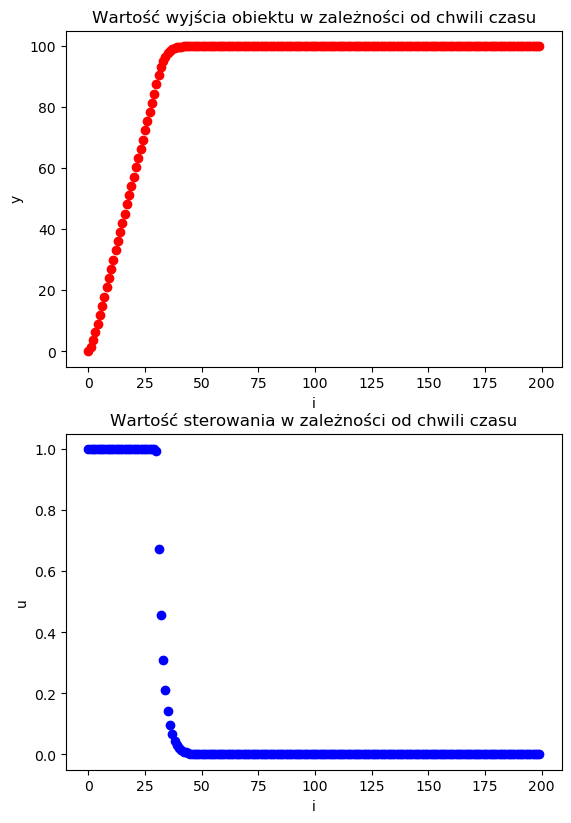
\includegraphics[width=\textwidth]{A_[0.1, 0.2, 0.1, 0.2, 0, 0.5, 0.1, 1, 0, 0, 1, 0, 0, 0, 0, 1]}
	\caption{Nasycone sterowanie}
	\label{fig:saturated}
\end{figure}

\section{Różne parametry regulatora}
Na kolejnych rysunkach \ref{fig:horizons_3_3}, \ref{fig:horizons_5_3}, \ref{fig:horizons_10_3},
\ref{fig:horizons_15_2}, \ref{fig:horizons_15_3}, \ref{fig:horizons_15_5}, \ref{fig:horizons_15_7},
\ref{fig:horizons_15_8} oraz \ref{fig:horizons_30_8} przedstawiono wpływ różnych parametrów regulatora MPC
na jakość sterowania oraz odpowiedzi układu regulacji. 
\begin{figure}[p]
    \centering
	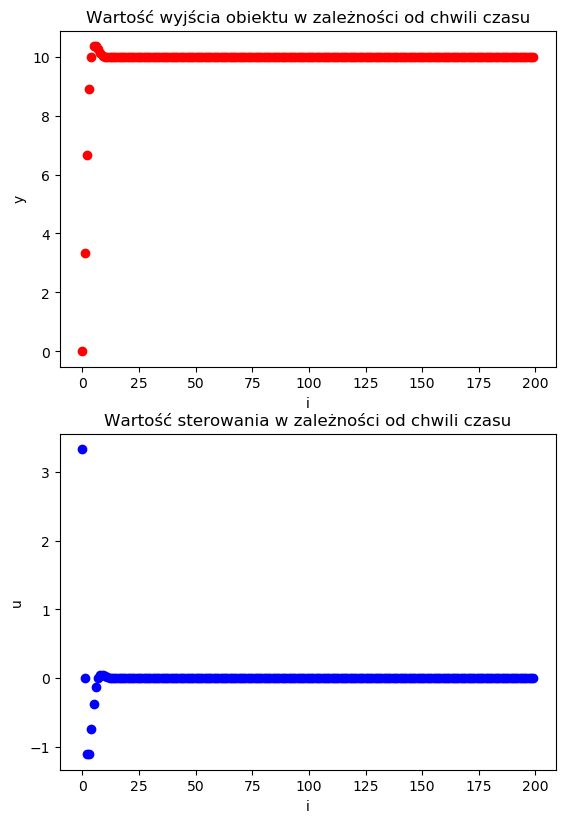
\includegraphics[width=\textwidth]{horizons_[3, 3]}
	\caption{Horyzont predykcji: 3, horyzont sterowań: 3}
	\label{fig:horizons_3_3}
\end{figure}

\begin{figure}[p]
    \centering
	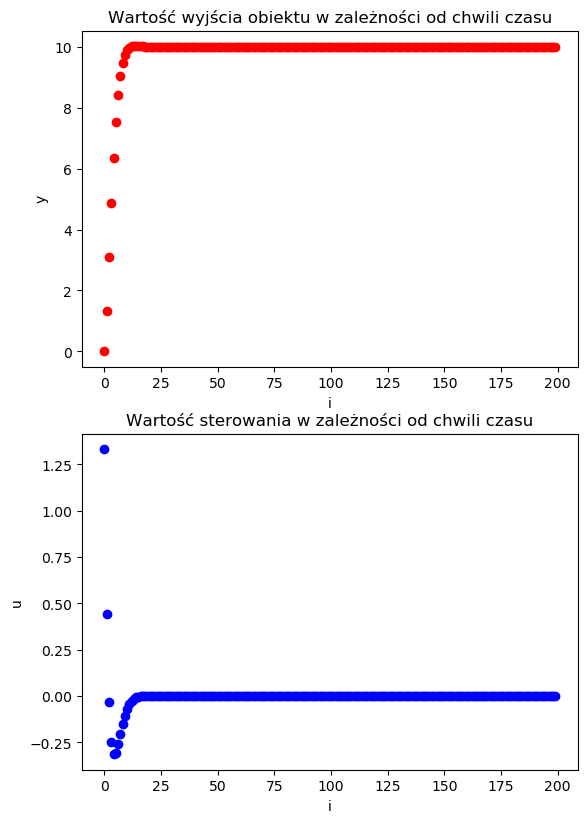
\includegraphics[width=\textwidth]{horizons_[5, 3]}
	\caption{Horyzont predykcji: 5, horyzont sterowań: 3}
	\label{fig:horizons_5_3}
\end{figure}

\begin{figure}[p]
    \centering
	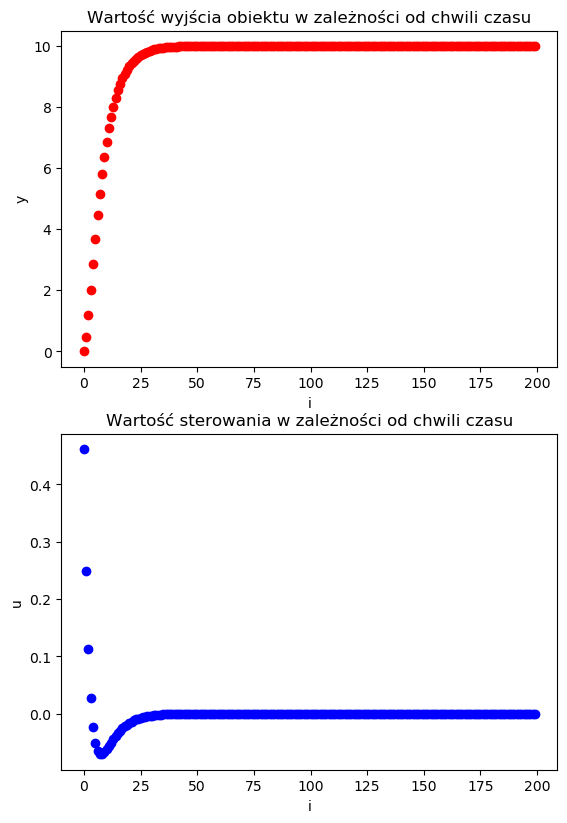
\includegraphics[width=\textwidth]{horizons_[10, 3]}
	\caption{Horyzont predykcji: 10, horyzont sterowań: 3}
	\label{fig:horizons_10_3}
\end{figure}

\begin{figure}[p]
    \centering
	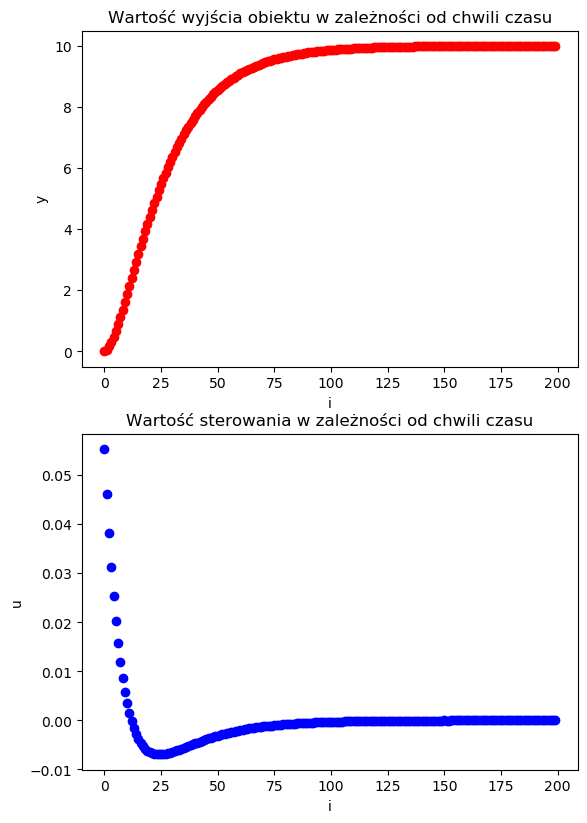
\includegraphics[width=\textwidth]{horizons_[15, 2]}
	\caption{Horyzont predykcji: 15, horyzont sterowań: 2}
	\label{fig:horizons_15_2}
\end{figure}

\begin{figure}[p]
    \centering
	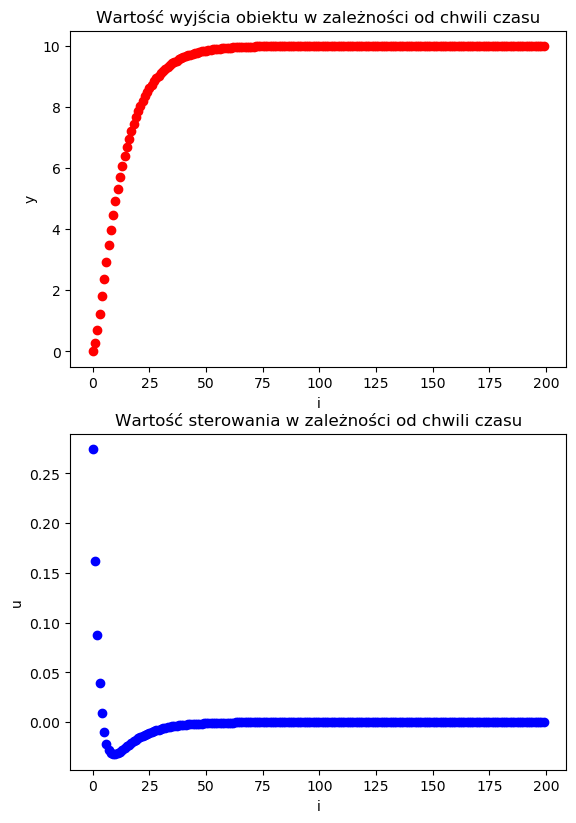
\includegraphics[width=\textwidth]{horizons_[15, 3]}
	\caption{Horyzont predykcji: 15, horyzont sterowań: 3}
	\label{fig:horizons_15_3}
\end{figure}

\begin{figure}[p]
    \centering
	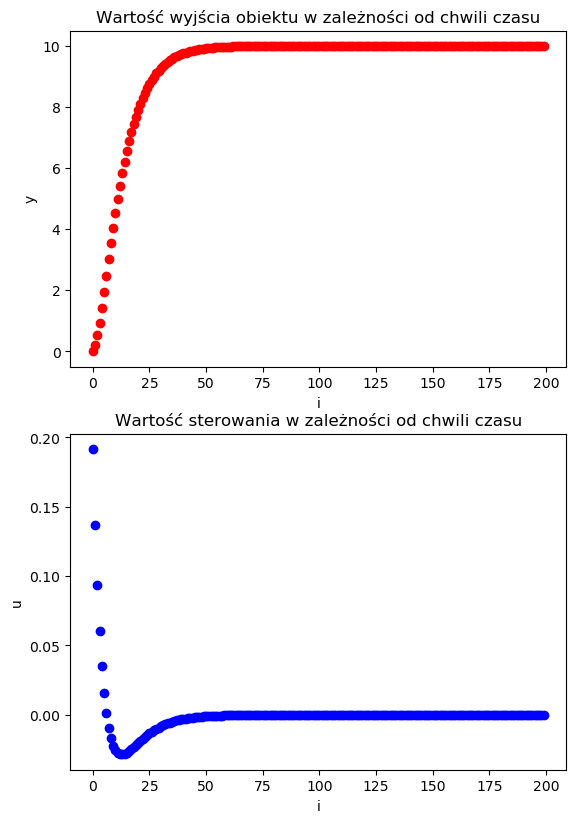
\includegraphics[width=\textwidth]{horizons_[15, 5]}
	\caption{Horyzont predykcji: 15, horyzont sterowań: 5}
	\label{fig:horizons_15_5}
\end{figure}

\begin{figure}[p]
    \centering
	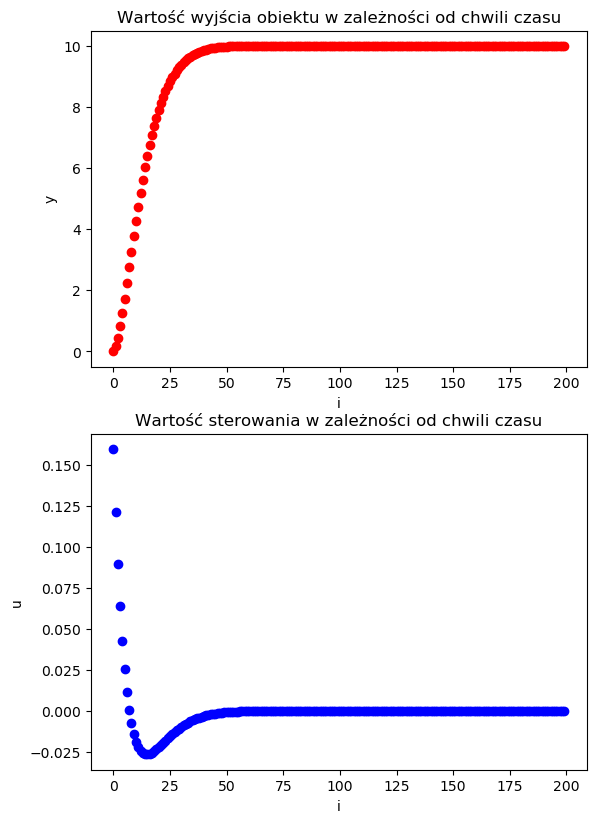
\includegraphics[width=\textwidth]{horizons_[15, 7]}
	\caption{Horyzont predykcji: 15, horyzont sterowań: 7}
	\label{fig:horizons_15_7}
\end{figure}

\begin{figure}[p]
    \centering
	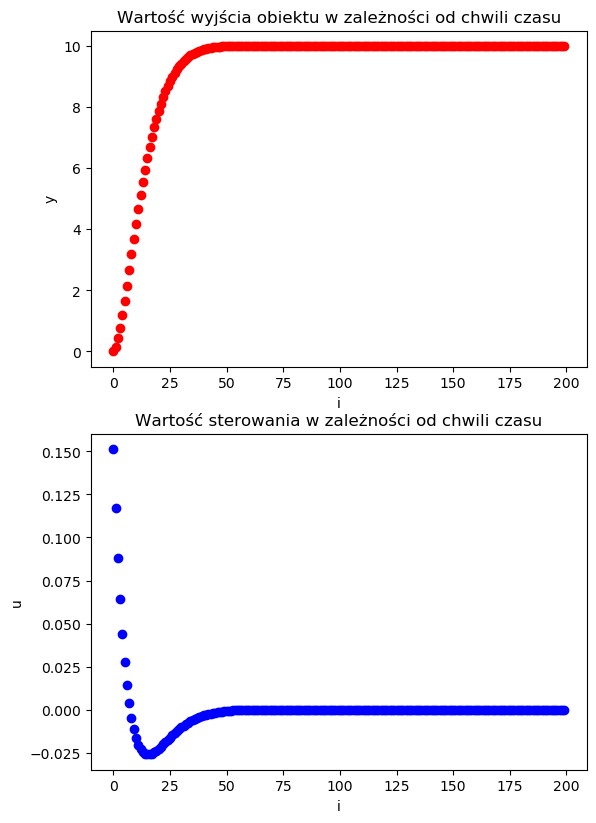
\includegraphics[width=\textwidth]{horizons_[15, 8]}
	\caption{Horyzont predykcji: 15, horyzont sterowań: 8}
	\label{fig:horizons_15_8}
\end{figure}

\begin{figure}[p]
    \centering
	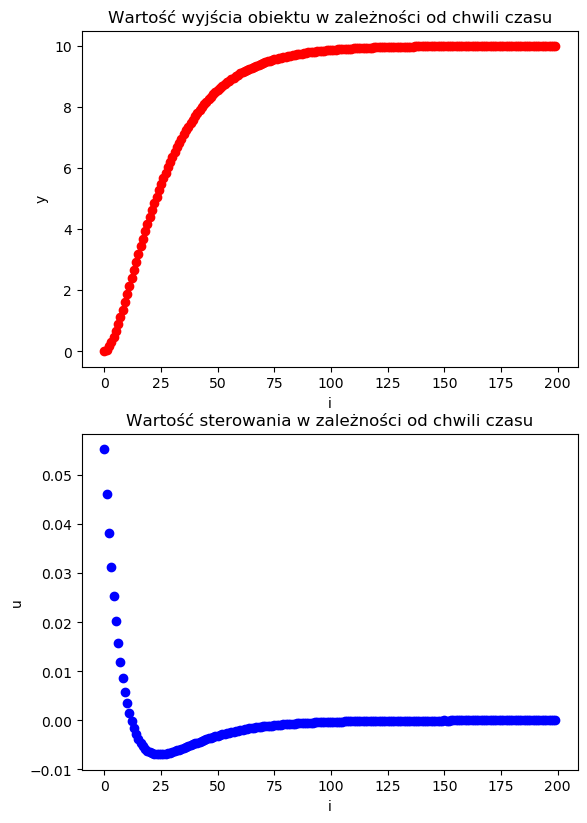
\includegraphics[width=\textwidth]{horizons_[30, 8]}
	\caption{Horyzont predykcji: 30, horyzont sterowań: 8}
	\label{fig:horizons_30_8}
\end{figure}

\chapter{Podsumowanie} \label{ch:summary}
\section{Wyniki}
Zebrane przykładowe wyniki pozwoliły na zapoznanie się z podstawowymi cechami regulacji
predykcyjnej. Wyciągnięto także następujące wnioski.

\section{Wnioski}
Realizacja postawionych w~rozdziale \ref{sec:assumptions} założeń pozwoliła na~sprawdzenie
wpływu horyzontu predykcji oraz sterowań na~jakość otrzymanej regulacji. Zbyt mały horyzont
predykcji w~badanym przypadku skutkował sporą amplitudą kolejnych początkowych sterowań. Zbyt
duży horyzont predykcji wpływał na~zwiększenie się opóźnienia w~układzie regulacji. Zwiększenie się
horyzontu sterowań było ściśle powiązane z~zwiększeniem się złożoności obliczeniowej problemu,
a przede wszystkim konieczności użycia większej ilości pamięci.
Ponadto potwierdzono cechę charakterystyczną sterowania predykcyjnego, a~mianowicie minimalizację
wartości pomiędzy kolejnymi sterowaniami. Im~horyzont predykcji był większy, tym owa różnica
była mniejsza.

\section{Pomysły na~rozwój projektu}
Istnieją dwie płaszczyzny, na~których można rozwinąć przygotowany projekt. Pierwsza z~nich dotyczy
doboru biblioteki do~obsługi rejestrów mikrokontrolera platformy STM. Jedną z~bardziej przyjaznych
użytkowniki alternatywnych opcji do~korzystania z~Cube'a jest otwartoźródłowy projekt
\textit{libopencm3}. Oferowane rozwiązania tejże biblioteki są~znacznie bardziej przejrzyste
oraz lepiej udokumentowane. Z~jej pomocą można bezproblemowo zastąpić komunikację opartą na
opisanym w~rozdziale \ref{sec:uart} pollingu przerwaniami systemowymi. Kolejnym aspektem
stricte programistycznym jest zmiana sposobu alokacji używanych w~rozwiązaniu macierzy z
dynamicznego na~statyczny. Przeniesienie wykonywania największej części obliczeń ze~sterty
na stos poprawiłoby w~znaczny sposób wydajność napisanego programu.

Drugą płaszczyzna jest związana z~zakresem badanych funkcjonalności regulatora MPC. Warte
rozważenia są~w~tym przypadku dwie możliwości rozwoju. Pierwsza z~nich zakłada rozszerzenie
możliwości pracy regulatora o~model nieliniowy przy pomocy techniki linearyzacji. Pozwoliłoby
to zweryfikować poprawność pracy zaimplementowanego algorytmu MPC na~szerszej dziedzinie
obiektów. Docelowym rozwiązaniem jest realizacja indetyfikacji obiektu oraz rozwiązywanie
zadania optymalizacji przy nieznanym modelu obiektu. 

\begin{appendices}
\chapter{Porównanie matlab stm}
\end{appendices}

\newpage

% Lists of objects
\listoffigures
\listoftables
\listoflistings

% Bibliography
\nocite{*}
\bibliographystyle{plplain}
\bibliography{references}

\end{document}
